\documentclass[11pt,oneside]{article}

\usepackage[a4paper,margin=26mm,headheight=15pt]{geometry}
\usepackage[T1]{fontenc}
\usepackage[utf8]{inputenc}
\IfFileExists{libertinus.sty}{\usepackage{libertinus}}{\usepackage{lmodern}}
\usepackage{microtype}
\usepackage{amsmath,amssymb,amsthm,mathtools}
\usepackage{bm}
\usepackage{booktabs,longtable,array,tabularx}
\usepackage{graphicx}
\usepackage{xcolor}
\usepackage{enumitem}
\usepackage{fancyhdr}
\usepackage{listings}
\usepackage{xurl}
\usepackage[hypertexnames=false]{hyperref}
\usepackage[nameinlink,noabbrev]{cleveref}

\definecolor{linkblue}{RGB}{25,75,135}
\definecolor{shadegray}{RGB}{246,247,249}
\definecolor{rulegray}{RGB}{195,201,208}
\hypersetup{
  colorlinks=true,
  linkcolor=linkblue,
  citecolor=linkblue,
  urlcolor=linkblue,
  pdftitle={Diagonal Polynomials and Dyadic Block Geometry in Repeated Thue--Morse Summation},
  pdfsubject={Exact diagonal laws, Sheffer recurrences, half-integer roots, and row geometry},
  pdfkeywords={Thue-Morse, Fabius function, repeated summation, diagonal polynomial, Sheffer sequence, Bell polynomial, dyadic block}
}

\pagestyle{fancy}
\fancyhf{}
\fancyhead[L]{\small Repeated Thue--Morse summation}
\fancyhead[R]{\small\nouppercase{\leftmark}}
\fancyfoot[C]{\thepage}
\renewcommand{\headrulewidth}{0.4pt}

\setcounter{secnumdepth}{3}
\setcounter{tocdepth}{2}
\setlength{\emergencystretch}{3em}
\allowdisplaybreaks
\numberwithin{equation}{section}
\setlist[itemize]{leftmargin=2em,itemsep=0.25em,topsep=0.4em}
\setlist[enumerate]{leftmargin=2.4em,itemsep=0.25em,topsep=0.4em}

\newtheorem{theorem}{Theorem}[section]
\newtheorem{proposition}[theorem]{Proposition}
\newtheorem{corollary}[theorem]{Corollary}
\newtheorem{lemma}[theorem]{Lemma}
\theoremstyle{definition}
\newtheorem{definition}[theorem]{Definition}
\newtheorem{algorithm}[theorem]{Algorithm}
\newtheorem{example}[theorem]{Example}
\theoremstyle{remark}
\newtheorem{remark}[theorem]{Remark}

\newcommand{\N}{\mathbb N}
\newcommand{\Nzero}{\mathbb N_0}
\newcommand{\Z}{\mathbb Z}
\newcommand{\Q}{\mathbb Q}
\newcommand{\eps}{\varepsilon}
\newcommand{\TM}{\operatorname{TM}}
\newcommand{\wt}{\operatorname{wt}_2}
\newcommand{\coeff}[2]{[z^{#1}]\,#2}
\newcommand{\rising}[2]{#1^{\overline{#2}}}
\newcommand{\falling}[2]{#1^{\underline{#2}}}
\newcommand{\nuTwo}{\nu_2}
\newcommand{\bigO}{\mathcal O}
\newcommand{\Diag}{D}
\newcommand{\Prefix}{T}
\newcommand{\Bell}{\mathcal B}
\newcommand{\stirlingfirst}[2]{\genfrac{[}{]}{0pt}{}{#1}{#2}}

\newenvironment{boxedsummary}{%
  \par\medskip\noindent\begin{center}\begin{minipage}{0.94\textwidth}%
  \hrule\vspace{0.7em}\small
}{%
  \vspace{0.7em}\hrule\end{minipage}\end{center}\medskip
}

\lstdefinestyle{code}{
  basicstyle=\ttfamily\small,
  backgroundcolor=\color{shadegray},
  frame=single,
  rulecolor=\color{rulegray},
  columns=fullflexible,
  keepspaces=true,
  showstringspaces=false,
  breaklines=true,
  xleftmargin=0.6em,
  xrightmargin=0.6em,
  aboveskip=0.8em,
  belowskip=0.8em
}
\lstset{style=code}

\title{\bfseries Diagonal Polynomials and Dyadic Block Geometry\\
       in Repeated Thue--Morse Summation}
\author{A proof-oriented research note for the \texttt{ProveIt} Fabius-function corpus}
\date{3 September 2026}

\begin{document}
\maketitle

\begin{abstract}
Consider the two-dimensional table specified by the signed Thue--Morse prefix
row and the weighted recurrence
\[
 s_{n,k}=\sum_{j=0}^{k-1}(k-j)s_{n-1,j}.
\]
The first visible diagonals are polynomial in the row index, but the supplied
code lists only eight such laws.  We derive the polynomial on every diagonal,
prove a complete generating-function description of the table, and explain
all dyadic acceleration rules in the code.

If \(r=k-n-1\ge0\), then
\[
 s_{n,n+1+r}=\Diag_r(n),\qquad
 \Diag_r(x)=\sum_{q=0}^{\lfloor r/2\rfloor}
 (-1)^{\wt(q)}
 \binom{2x+r-2q-1}{r-2q}.
\]
Thus \(\Diag_r\) has exact degree \(r\), leading coefficient \(2^r/r!\),
is integer-valued on the half-integer lattice, and admits Stirling,
Bell-polynomial, Sheffer, differential, half-step, and ruler-function
recurrences.  Its nonnegative half-integer zeros have an exact modular
classification: \(\Diag_r(m/2)=0\) precisely when the residue of \(r\) modulo
\(2^{m+1}\) lies in the final \(m+1\) positions of the block.  Negative
half-integer values are finite backward differences of the signed
Thue--Morse sequence.

For each fixed row \(n\), the entire infinite sequence is a signed repetition
of one nonnegative block of length \(2^{2n+1}\).  We prove its support,
circular reflection, complement law, exact central plateau, maximum, total
mass, multiplicities, and number of distinct values.  The same argument gives
a finite-block theorem for every order of iterated summation, resolving in one
factorization the periodicity and extremal patterns observed in the earlier
computational question.  A fully commented Python program performs exact
checks and generates the accompanying profile figure.
\end{abstract}

\tableofcontents
\clearpage

\section{Problem, conventions, and main answer}

\subsection{The table}

Let
\begin{equation}
  \eps_q=(-1)^{\wt(q)},\qquad q\in\Nzero,
  \label{eq:tm-sign}
\end{equation}
where \(\wt(q)\) is the number of ones in the binary expansion of \(q\).
This is the signed Thue--Morse sequence.  Throughout the paper, \(n\) and
\(k\) are nonnegative integers.  The code in the question is read as defining
\(s_{n,k}\) with the triangular initial condition \(s_{n,k}=0\) for
\(k\le n\), the signed-prefix row at \(n=0\), and the fallback recurrence
\begin{equation}
  s_{n,k}=\sum_{j=0}^{k-1}(k-j)s_{n-1,j},\qquad n\ge1.
  \label{eq:weighted-recurrence}
\end{equation}
The symmetry branches and the first eight diagonal formulas are computational
shortcuts.  We will derive them rather than assume them.

The repository's Thue--Morse atlas proves the exact prefix collapse, the
iterated-prefix convolution and generating function, terminal dyadic zero
runs, and signed reversal, with explicit Lean crosswalks for those statements
\cite{ReshetnikovAtlas}.  The present note reorganizes those ingredients around
the two indices \((n,k)\), and develops the fixed-diagonal polynomial calculus.
No priority claim is made for identities that follow from standard formal
power-series manipulations.

\subsection{The diagonal coordinate}

The first nonzero entry of row \(n\) occurs at \(k=n+1\).  It is therefore
natural to set
\begin{equation}
  r=k-n-1.
  \label{eq:r-coordinate}
\end{equation}
The visible diagonal \(k-n=d\) in the original table corresponds to
\(r=d-1\).  We reserve \(\Diag_r(x)\) for the polynomial attached to this
offset.

\begin{boxedsummary}
\textbf{Closed form for an arbitrary diagonal.}
For every \(r\ge0\), define
\begin{equation}
 \boxed{
 \Diag_r(x)=
 \sum_{q=0}^{\lfloor r/2\rfloor}
 \eps_q\binom{2x+r-2q-1}{r-2q}
 =\sum_{q=0}^{\lfloor r/2\rfloor}
 \eps_q\frac{\rising{2x}{r-2q}}{(r-2q)!}.}
 \label{eq:main-diagonal}
\end{equation}
Then
\begin{equation}
 \boxed{
 s_{n,k}=\begin{cases}
 0,&k\le n,\\[2mm]
 \Diag_{k-n-1}(n),&k\ge n+1.
 \end{cases}}
 \label{eq:main-table-answer}
\end{equation}
Equivalently, the polynomial on the original diagonal \(d=k-n\ge1\) is
\begin{equation}
 \boxed{
 P_d(x)=\Diag_{d-1}(x)=
 \sum_{q=0}^{\lfloor(d-1)/2\rfloor}
 \eps_q\binom{2x+d-2q-2}{d-2q-1}.}
 \label{eq:main-d-answer}
\end{equation}
It has degree \(d-1\) and leading coefficient \(2^{d-1}/(d-1)!\).
\end{boxedsummary}

Formula \eqref{eq:main-diagonal} is finite and exact.  It is not an
interpolation guessed from numerical rows: it follows coefficientwise from a
single generating function, and hence applies to every row and every
nonnegative column.

\subsection{Summary of the structural results}

The article proves the following additional facts.

\begin{enumerate}
\item The row generating function is
\[
 A_n(z):=\sum_{k\ge0}s_{n,k}z^k
 =\frac{z^{n+1}E(z^2)}{(1-z)^{2n}}
 =\frac{z^{n+1}E(z)}{(1-z)^{2n+1}},
\]
where \(E(z)=\sum_{q\ge0}\eps_qz^q\).

\item The shifted row is exactly an odd-order iterated prefix:
\[
 s_{n,n+1+r}=\Prefix_r^{(2n+1)}.
\]
Thus the diagonal polynomial interpolates a fixed coefficient as the order of
summation varies.

\item The sequence \(p_r(x)=r!\Diag_r(x)\) is Sheffer for
\[
 E(z^2)\exp\!\bigl(-2x\log(1-z)\bigr).
\]
In particular,
\[
 \Diag_r(x)-\Diag_r(x-\tfrac12)=\Diag_{r-1}(x)
\]
and
\[
 r\Diag_r(x)=\sum_{m=1}^r
 \bigl(2x+2-2^{\nuTwo(m)+1}\bigr)\Diag_{r-m}(x).
\]

\item For \(m\ge0\),
\[
 \Diag_r(m/2)=0
 \iff
 r\bmod 2^{m+1}\in
 \{2^{m+1}-(m+1),\ldots,2^{m+1}-1\}.
\]

\item A row has block length \(L=2^{2n+1}\), block maximum
\(M_n=2^{\binom{2n}{2}}\), exactly \(2n+1\) zero positions, exactly
\(2n+1\) maximum positions, and
\(2^{2n}-2n+1\) distinct absolute values.  Every nonextreme value occurs
exactly twice.
\end{enumerate}

\section{Signed Thue--Morse prefixes and formal products}

\subsection{The lacunary product}

The binary recursions
\begin{equation}
  \eps_{2q}=\eps_q,
  \qquad
  \eps_{2q+1}=-\eps_q
  \label{eq:tm-recursion}
\end{equation}
imply the formal product identity
\begin{equation}
 E(z):=\sum_{q\ge0}\eps_qz^q
 =\prod_{j\ge0}(1-z^{2^j}).
 \label{eq:E-product}
\end{equation}
Every coefficient of the infinite product stabilizes after finitely many
factors, so \eqref{eq:E-product} is valid in \(\Z[[z]]\); no analytic
convergence is required.  Separating the first factor gives the Mahler
relation
\begin{equation}
 E(z)=(1-z)E(z^2).
 \label{eq:Mahler}
\end{equation}
These identities are standard in the theory of automatic sequences
\cite{AlloucheShallit}; they are also the algebraic engine of the repository's
Fabius--Rvachev development \cite{ReshetnikovAtlas}.

\subsection{Exclusive and inclusive prefixes}

Define the exclusive prefix
\begin{equation}
 S(k)=\sum_{j=0}^{k-1}\eps_j,
 \qquad S(0)=0.
 \label{eq:exclusive-prefix}
\end{equation}
Pairing \(\eps_{2q}+\eps_{2q+1}=0\) gives
\begin{equation}
 S(2q)=0,
 \qquad
 S(2q+1)=\eps_q.
 \label{eq:prefix-collapse}
\end{equation}
Consequently,
\begin{equation}
 \sum_{k\ge0}S(k)z^k
 =zE(z^2)
 =\frac{zE(z)}{1-z}.
 \label{eq:prefix-gf}
\end{equation}
This is precisely the \(n=0\) row encoded by the supplied Wolfram Language
branches.

For comparison with repeated summation, define inclusive iterates
\begin{equation}
 \Prefix_r^{(0)}=\eps_r,
 \qquad
 \Prefix_r^{(h+1)}=\sum_{j=0}^{r}\Prefix_j^{(h)}.
 \label{eq:inclusive-prefix-definition}
\end{equation}
One summation multiplies an ordinary generating function by \((1-z)^{-1}\),
so
\begin{equation}
 \sum_{r\ge0}\Prefix_r^{(h)}z^r
 =\frac{E(z)}{(1-z)^h}.
 \label{eq:inclusive-prefix-gf}
\end{equation}
For \(h\ge1\), coefficient extraction yields
\begin{equation}
 \Prefix_r^{(h)}
 =\sum_{j=0}^{r}
 \binom{r-j+h-1}{h-1}\eps_j.
 \label{eq:inclusive-prefix-convolution}
\end{equation}
Bertazzon's construction of a solution to a Thue--Morse integral equation uses
these repeated sums and their dyadic block coefficients in essentially this
form \cite{Bertazzon2012}.

\section{Generating function of the complete two-dimensional table}

\subsection{The weighted recurrence as two summations}

Let
\begin{equation}
 A_n(z)=\sum_{k\ge0}s_{n,k}z^k.
 \label{eq:row-gf-definition}
\end{equation}
The kernel in \eqref{eq:weighted-recurrence} has generating function
\begin{equation}
 \sum_{m\ge1}m z^m=\frac{z}{(1-z)^2}.
 \label{eq:kernel-gf}
\end{equation}
Thus \eqref{eq:weighted-recurrence} is convolution by the coefficient sequence
\(1,2,3,\ldots\), or equivalently two discrete antiderivatives together with
a one-step shift.

\begin{theorem}[Exact row generating function]
For every \(n\ge0\),
\begin{equation}
 \boxed{
 A_n(z)=
 \left(\frac{z}{(1-z)^2}\right)^n zE(z^2)
 =\frac{z^{n+1}E(z^2)}{(1-z)^{2n}}
 =\frac{z^{n+1}E(z)}{(1-z)^{2n+1}}.}
 \label{eq:row-gf}
\end{equation}
\end{theorem}

\begin{proof}
Equation \eqref{eq:prefix-gf} gives \(A_0(z)=zE(z^2)\).  Multiplying by
\eqref{eq:kernel-gf} implements the recurrence once, so induction gives the
first two expressions.  The last follows from the Mahler identity
\eqref{eq:Mahler}.
\end{proof}

The triangular zero region is now automatic: \(A_n\) is divisible by
\(z^{n+1}\).  More importantly, shifting by this monomial identifies each row
with a standard iterated-prefix sequence.

\begin{corollary}[Rows are odd-order iterated prefixes]
For every \(n,r\ge0\),
\begin{equation}
 \boxed{s_{n,n+1+r}=\Prefix_r^{(2n+1)}.}
 \label{eq:row-prefix-identification}
\end{equation}
Equivalently,
\begin{equation}
 s_{n,n+1+r}
 =\sum_{j=0}^{r}\eps_j\binom{2n+r-j}{2n}.
 \label{eq:row-prefix-convolution}
\end{equation}
\end{corollary}

\begin{proof}
After removing \(z^{n+1}\) from \eqref{eq:row-gf}, the remaining generating
function is \(E(z)/(1-z)^{2n+1}\), which is
\eqref{eq:inclusive-prefix-gf} with \(h=2n+1\).
\end{proof}

This relation also identifies the absolute values in the earlier question on
periodic iterated Thue--Morse sums.  With the notation used there,
\begin{equation}
 |s_{n,n+1+r}|=u_r^{(2n)}.
 \label{eq:mathse-map}
\end{equation}
The row index \(n\) therefore advances the summation order by two.

\subsection{Two bivariate generating functions}

Summing \eqref{eq:row-gf} over the row index gives a compact encoding of the
whole array.

\begin{proposition}[Bivariate table generating function]
As a formal power series in \(u\) with coefficients in \(\Z[[z]]\),
\begin{equation}
 \boxed{
 \sum_{n\ge0}\sum_{k\ge0}s_{n,k}u^nz^k
 =\frac{z(1-z)^2E(z^2)}{(1-z)^2-uz}.}
 \label{eq:bivariate-table}
\end{equation}
For the diagonal array \(\Diag_r(n)=s_{n,n+1+r}\),
\begin{equation}
 \boxed{
 \sum_{n\ge0}\sum_{r\ge0}\Diag_r(n)u^nz^r
 =\frac{(1-z)^2E(z^2)}{(1-z)^2-u}.}
 \label{eq:bivariate-diagonal}
\end{equation}
\end{proposition}

\begin{proof}
Both formulas are geometric sums.  For example,
\[
 \sum_{n\ge0}u^nA_n(z)
 =zE(z^2)\sum_{n\ge0}
 \left(\frac{uz}{(1-z)^2}\right)^n.
\]
Removing the shift \(z^{n+1}\) before summing gives
\eqref{eq:bivariate-diagonal}.
\end{proof}

\section{Why fixed-index iterated sums are polynomials}

The polynomial phenomenon is not peculiar to Thue--Morse.  It is a universal
property of repeated summation, sharpened here by the Mahler factorization.

\subsection{A general summation-order polynomial}

Let \(a_0,a_1,\ldots\) be any sequence over a characteristic-zero field and
let
\[
 A(z)=\sum_{j\ge0}a_jz^j.
\]
For an integer \(h\ge0\), write \(U_r^{(h)}\) for the \(h\)-fold inclusive
sum, so its generating function is \(A(z)/(1-z)^h\).

\begin{theorem}[Polynomiality in the summation order]
For each fixed \(r\ge0\), the coefficient
\begin{equation}
 U_r(h):=\coeff{r}{\frac{A(z)}{(1-z)^h}}
 \label{eq:general-U}
\end{equation}
extends from \(h\in\Nzero\) to the polynomial
\begin{equation}
 \boxed{
 U_r(h)=\sum_{j=0}^{r}a_j
 \binom{h+r-j-1}{r-j}.}
 \label{eq:general-order-polynomial}
\end{equation}
Its degree is at most \(r\), and is exactly \(r\) if \(a_0\ne0\), with
leading coefficient \(a_0/r!\).
\end{theorem}

\begin{proof}
Expand
\[
 (1-z)^{-h}=\sum_{m\ge0}\binom{h+m-1}{m}z^m
\]
formally and take the Cauchy coefficient at \(z^r\).  For fixed \(m\), the
generalized binomial coefficient is a polynomial in \(h\) of degree \(m\).
Only the term \(j=0\), for which \(m=r\), can contribute degree \(r\).
\end{proof}

The value at \(h=0\) is included: the generalized binomial vanishes for
positive lower index and upper index one smaller, leaving \(U_r(0)=a_r\).
This polynomial continuation is therefore canonical, not an arbitrary fit.

\subsection{Mahler deflation and sparse diagonals}

Many automatic sequences have a functional factorization that compresses the
sum \eqref{eq:general-order-polynomial}.

\begin{theorem}[A general deflation principle]
Suppose
\begin{equation}
 A(z)=(1-z)^cB(z^b),
 \qquad
 B(z)=\sum_{q\ge0}b_qz^q,
 \label{eq:general-deflation-hypothesis}
\end{equation}
where \(b\ge2\) and \(c\in\Z\).  Then
\begin{equation}
 \boxed{
 U_r(h)=
 \sum_{q=0}^{\lfloor r/b\rfloor}b_q
 \binom{h-c+r-bq-1}{r-bq}.}
 \label{eq:general-deflation}
\end{equation}
Thus only one residue class modulo \(b\) of coefficient degrees occurs.
\end{theorem}

\begin{proof}
Substitute \eqref{eq:general-deflation-hypothesis} into
\eqref{eq:general-U}:
\[
 \frac{A(z)}{(1-z)^h}=B(z^b)(1-z)^{-(h-c)}.
\]
The term \(b_qz^{bq}\) leaves coefficient degree \(r-bq\) in the binomial
series.
\end{proof}

For Thue--Morse, \eqref{eq:Mahler} has \(b=2\), \(c=1\), and \(B=E\).
Therefore
\begin{equation}
 \Prefix_r^{(h)}
 =\sum_{q=0}^{\lfloor r/2\rfloor}
 \eps_q\binom{h+r-2q-2}{r-2q}.
 \label{eq:prefix-order-polynomial}
\end{equation}
Since the table uses \(h=2n+1\), formula \eqref{eq:main-diagonal} follows
immediately.  This proves the main answer \eqref{eq:main-table-answer}.

\begin{remark}[Interpretation]
For a fixed coefficient index \(r\), \(\Diag_r(x)\) is the polynomial
continuation of the \(h\)-fold signed Thue--Morse prefix under the affine
change \(h=2x+1\):
\begin{equation}
 \Diag_r(x)=\Prefix_r^{(2x+1)}
 \quad\text{in the sense of polynomial continuation in }h.
 \label{eq:polynomial-interpolation-interpretation}
\end{equation}
At integer \(x=n\), this is exactly the row identity
\eqref{eq:row-prefix-identification}.
\end{remark}

\section{The diagonal polynomials}

\subsection{First examples and agreement with the supplied code}

Expanding \eqref{eq:main-diagonal} gives the following first eight members.
They are exactly the eight explicit branches in the question after replacing
\(x\) by \(n\) and \(r\) by \(k-n-1\).

\begin{align}
 \Diag_0(x)&=1,\label{eq:D0}\\
 \Diag_1(x)&=2x,\label{eq:D1}\\
 \Diag_2(x)&=(x+1)(2x-1),\label{eq:D2}\\
 \Diag_3(x)&=\frac{2}{3}x(x+2)(2x-1),\label{eq:D3}\\
 \Diag_4(x)&=\frac{1}{6}
 (4x^4+12x^3-x^2-3x-6),\label{eq:D4}\\
 \Diag_5(x)&=\frac{1}{15}x(x-1)
 (4x^3+24x^2+39x+34),\label{eq:D5}\\
 \Diag_6(x)&=\frac{1}{90}(x-1)(x+1)(2x-1)
 (4x^3+32x^2+75x+90),\label{eq:D6}\\
 \Diag_7(x)&=\frac{1}{315}x(x-1)(x+2)(2x-1)
 (4x^3+40x^2+123x+192).\label{eq:D7}
\end{align}

The formula separates two kinds of structure.  The rising-factorial terms
control degree and coefficient growth, while the digital signs \(\eps_q\)
insert corrections only at degree gaps \(2q\).  This separation becomes
transparent in the monomial coefficient formula below.

\subsection{Degree, leading layers, and integrality}

\begin{theorem}[Basic shape]
For \(r\ge0\), the polynomial \(\Diag_r\) has the following properties.
\begin{enumerate}
\item \(\deg \Diag_r=r\) and
\begin{equation}
 [x^r]\Diag_r(x)=\frac{2^r}{r!}.
 \label{eq:leading-coefficient}
\end{equation}
\item \(r!\Diag_r(x)\in\Z[x]\).
\item \(\Diag_r(x)\in\Z\) whenever \(2x\in\Z\); in particular, every
integer and half-integer value is integral.
\item At the origin,
\begin{equation}
 \Diag_r(0)=
 \begin{cases}
 \eps_{r/2},&r\text{ even},\\
 0,&r\text{ odd}.
 \end{cases}
 \label{eq:origin-values}
\end{equation}
Thus every odd-indexed diagonal polynomial is divisible by \(x\).
\end{enumerate}
\end{theorem}

\begin{proof}
In \eqref{eq:main-diagonal}, the \(q=0\) term has degree \(r\) and leading
coefficient \(2^r/r!\); every other term has degree at most \(r-2\).  After
multiplication by \(r!\), each summand is an integer multiple of
\(\rising{2x}{r-2q}\), which belongs to \(\Z[x]\).  If \(2x=t\in\Z\), then
\(\binom{t+m-1}{m}\in\Z\) for every \(m\ge0\), including negative \(t\) by
the generalized-binomial identity.  Finally, setting \(x=0\) kills every
positive rising factorial, leaving only the term with \(r-2q=0\), when one
exists.
\end{proof}

Let \(\stirlingfirst{m}{\ell}\) denote the unsigned Stirling number of
the first kind, characterized by
\begin{equation}
 \rising{y}{m}=\sum_{\ell=0}^{m}
 \stirlingfirst{m}{\ell}y^\ell.
 \label{eq:stirling-rising}
\end{equation}

\begin{theorem}[All monomial coefficients]
For \(0\le\ell\le r\),
\begin{equation}
 \boxed{
 [x^\ell]\Diag_r(x)=
 2^\ell
 \sum_{q=0}^{\lfloor(r-\ell)/2\rfloor}
 \eps_q\frac{\stirlingfirst{r-2q}{\ell}}{(r-2q)!}.}
 \label{eq:all-monomial-coefficients}
\end{equation}
Consequently, the coefficient of \(x^{r-a}\) depends only on
\(\eps_0,\ldots,\eps_{\lfloor a/2\rfloor}\).
\end{theorem}

\begin{proof}
Insert \eqref{eq:stirling-rising} into the second form of
\eqref{eq:main-diagonal} and compare powers of \(x\).  A term of degree
\(r-2q\) can contribute to \(x^\ell\) only if \(q\le(r-\ell)/2\).
\end{proof}

The first three degree layers are especially simple.  For \(r\ge3\),
\begin{equation}
 \boxed{
 \Diag_r(x)=
 \frac{2^r}{r!}x^r
 +\frac{2^{r-2}}{(r-2)!}x^{r-1}
 +\frac{2^{r-2}(3r^2-7r-22)}{24(r-2)!}x^{r-2}
 +\bigO(x^{r-3}).}
 \label{eq:top-three-layers}
\end{equation}
For fixed \(r\), this is also the large-row asymptotic shape of the diagonal
entry \(s_{n,n+1+r}\) as \(n\to\infty\).

\begin{proof}[Derivation of \eqref{eq:top-three-layers}]
The leading term was already established.  For degree \(r-1\), only \(q=0\)
contributes, and
\(
\stirlingfirst{r}{r-1}=\binom r2
\).
For degree \(r-2\), use
\[
 \stirlingfirst{r}{r-2}
 =\frac{r(r-1)(r-2)(3r-1)}{24}
\]
and include the leading coefficient of the \(q=1\) term, whose sign is
\(\eps_1=-1\).  Straight simplification gives the displayed coefficient.
\end{proof}

\subsection{Finite-product and inclusion--exclusion forms}

Although \(E(z^2)\) is an infinite product, only finitely many factors can
affect \(\Diag_r\).  If \(J=\lfloor\log_2r\rfloor\) for \(r\ge1\), then
\begin{equation}
 \Diag_r(x)=
 \coeff{r}{
 \frac{\prod_{j=1}^{J}(1-z^{2^j})}{(1-z)^{2x}}}.
 \label{eq:finite-product-diagonal}
\end{equation}
Equivalently, writing \(w(S)=\sum_{j\in S}2^j\),
\begin{equation}
 \Diag_r(x)=
 \sum_{\substack{S\subseteq\{1,\ldots,J\}\\w(S)\le r}}
 (-1)^{|S|}
 \binom{2x+r-w(S)-1}{r-w(S)}.
 \label{eq:subset-diagonal}
\end{equation}
The unique binary representation of each even number identifies
\eqref{eq:subset-diagonal} with \eqref{eq:main-diagonal}.

\section{Sheffer structure and efficient recurrences}

\subsection{A Sheffer family}

Define the scaled polynomials
\begin{equation}
 p_r(x)=r!\Diag_r(x).
 \label{eq:p-def}
\end{equation}
Then the ordinary generating function in \(\Diag_r\) is at the same time the
exponential generating function in \(p_r\):
\begin{equation}
 \sum_{r\ge0}\frac{p_r(x)}{r!}z^r
 =\sum_{r\ge0}\Diag_r(x)z^r
 =E(z^2)\exp\!\bigl(-2x\log(1-z)\bigr).
 \label{eq:Sheffer-egf}
\end{equation}
Thus \(p_r\) is a Sheffer sequence for the pair
\begin{equation}
 A(z)=E(z^2),
 \qquad
 f(z)=-2\log(1-z).
 \label{eq:Sheffer-pair}
\end{equation}
The terminology and standard operator calculus may be found, for example, in
Roman's treatment of the umbral calculus \cite{Roman1984}.  We derive every
identity needed here directly from \eqref{eq:Sheffer-egf}.

\subsection{Half-step lowering}

\begin{theorem}[Half-step recurrence]
With the convention \(\Diag_{-1}=0\),
\begin{equation}
 \boxed{
 \Diag_r(x)-\Diag_r(x-\tfrac12)=\Diag_{r-1}(x),
 \qquad r\ge0.}
 \label{eq:half-step}
\end{equation}
Equivalently, for \(p_r=r!\Diag_r\),
\begin{equation}
 \bigl(1-e^{-\frac12\partial_x}\bigr)p_r(x)
 =r p_{r-1}(x).
 \label{eq:delta-operator}
\end{equation}
\end{theorem}

\begin{proof}
Let
\[
 G_x(z)=\sum_{r\ge0}\Diag_r(x)z^r
 =E(z^2)(1-z)^{-2x}.
\]
Then \(G_{x-1/2}(z)=(1-z)G_x(z)\), so
\(G_x-G_{x-1/2}=zG_x\).  Compare coefficients.
\end{proof}

This identity is unusually useful: it says that a half-unit backward
difference in the row parameter lowers the diagonal index by one.  Iterating,
\begin{equation}
 \sum_{j=0}^{a}(-1)^j\binom aj
 \Diag_r\!\left(x-\frac j2\right)
 =\Diag_{r-a}(x),
 \qquad a\ge0.
 \label{eq:iterated-half-step}
\end{equation}

\subsection{Differentiation and addition}

\begin{theorem}[Differential recurrence]
For \(r\ge1\),
\begin{equation}
 \boxed{
 \Diag_r'(x)=2\sum_{j=1}^{r}\frac{\Diag_{r-j}(x)}{j}.}
 \label{eq:differential-recurrence}
\end{equation}
\end{theorem}

\begin{proof}
Differentiate \(G_x(z)\) with respect to \(x\):
\[
 \partial_xG_x(z)=-2\log(1-z)G_x(z)
 =2\left(\sum_{j\ge1}\frac{z^j}{j}\right)G_x(z).
\]
Compare coefficients.
\end{proof}

\begin{theorem}[Addition law]
For arbitrary \(x,y\),
\begin{equation}
 \boxed{
 \Diag_r(x+y)=\sum_{j=0}^{r}
 \Diag_{r-j}(x)\binom{2y+j-1}{j}.}
 \label{eq:addition-law}
\end{equation}
\end{theorem}

\begin{proof}
Factor \(G_{x+y}(z)=G_x(z)(1-z)^{-2y}\) and take the coefficient of \(z^r\).
\end{proof}

The half-step identity is the specialization \(y=-1/2\) after moving terms.
The addition law also makes clear that translation in \(x\) is triangular in
the diagonal index.

\subsection{The ruler-function recurrence}

The most efficient recurrence for generating many diagonal polynomials comes
from the logarithm of \(G_x\).  Recall that \(\nuTwo(m)\) is the exponent of
\(2\) in \(m\).

\begin{lemma}[Ruler logarithm]
One has
\begin{equation}
 \boxed{
 \log G_x(z)=\sum_{m\ge1}
 \frac{c_m(x)}{m}z^m,
 \qquad
 c_m(x)=2x+2-2^{\nuTwo(m)+1}.}
 \label{eq:ruler-logarithm}
\end{equation}
\end{lemma}

\begin{proof}
The denominator contributes
\(-2x\log(1-z)=2x\sum_{m\ge1}z^m/m\).  On the other hand,
\[
 \log E(z^2)
 =\sum_{j\ge1}\log(1-z^{2^j})
 =-\sum_{j\ge1}\sum_{a\ge1}\frac{z^{a2^j}}a.
\]
For fixed \(m\), the divisors \(2^j\mid m\) with \(j\ge1\) contribute
\[
 -\frac1m\sum_{j=1}^{\nuTwo(m)}2^j
 =-\frac{2^{\nuTwo(m)+1}-2}{m}.
\]
Adding the two parts gives \eqref{eq:ruler-logarithm}.
\end{proof}

\begin{theorem}[Ruler recurrence]
The diagonal polynomials satisfy
\begin{equation}
 \boxed{
 \Diag_0(x)=1,
 \qquad
 r\Diag_r(x)=\sum_{m=1}^{r}
 \bigl(2x+2-2^{\nuTwo(m)+1}\bigr)\Diag_{r-m}(x).}
 \label{eq:ruler-recurrence}
\end{equation}
\end{theorem}

\begin{proof}
Differentiate \(G_x(z)=\exp(\sum c_mz^m/m)\) with respect to \(z\):
\[
 zG_x'(z)=G_x(z)\sum_{m\ge1}c_m(x)z^m.
\]
Coefficient comparison gives the recurrence.
\end{proof}

The values \(2^{\nuTwo(m)}\) form the classical ruler sequence.  Hence all
digital dependence in this polynomial recurrence enters through a one-line
valuation statistic rather than explicit binary digit sums.

\subsection{Bell-polynomial form}

Let \(\Bell_r(y_1,\ldots,y_r)\) be the complete exponential Bell polynomial,
defined by
\begin{equation}
 \exp\left(\sum_{m\ge1}y_m\frac{z^m}{m!}\right)
 =\sum_{r\ge0}\Bell_r(y_1,\ldots,y_r)\frac{z^r}{r!}.
 \label{eq:Bell-definition}
\end{equation}
Then \eqref{eq:ruler-logarithm} gives an immediate closed form.

\begin{corollary}[Bell-polynomial representation]
\begin{equation}
 \boxed{
 \Diag_r(x)=\frac1{r!}
 \Bell_r\bigl(0!c_1(x),1!c_2(x),\ldots,(r-1)!c_r(x)\bigr),}
 \label{eq:Bell-form}
\end{equation}
where \(c_m(x)=2x+2-2^{\nuTwo(m)+1}\).
\end{corollary}

Bell polynomials provide determinant, partition, and recurrence formulas
through standard identities \cite{Comtet1974}.  In computation,
\eqref{eq:ruler-recurrence} is usually simpler, while \eqref{eq:Bell-form}
provides the cleanest conceptual packaging.

\section{Exact half-integer roots and factor patterns}

\subsection{Nonnegative half-integers}

The striking linear factors in the first displayed polynomials are not
accidental.  They are the visible part of an exact modular zero theorem.

\begin{theorem}[Complete nonnegative half-integer zero criterion]
Let \(r,m\in\Nzero\), put
\begin{equation}
 h=m+1,
 \qquad
 L=2^h.
 \label{eq:half-root-hL}
\end{equation}
Then
\begin{equation}
 \boxed{
 \Diag_r(m/2)=0
 \iff
 r\bmod L\in\{L-h,L-h+1,\ldots,L-1\}.}
 \label{eq:half-root-criterion}
\end{equation}
Equivalently,
\begin{equation}
 (2x-m)\mid\Diag_r(x)\quad\text{in }\Q[x]
 \iff
 r\bmod 2^{m+1}\ge2^{m+1}-(m+1).
 \label{eq:factor-criterion}
\end{equation}
These are exactly all zeros of \(\Diag_r\) on
\(\{0,\tfrac12,1,\tfrac32,\ldots\}\).
\end{theorem}

\begin{proof}
At \(x=m/2\), equation \eqref{eq:polynomial-interpolation-interpretation}
gives
\[
 \Diag_r(m/2)=\Prefix_r^{(m+1)}=\Prefix_r^{(h)}.
\]
Factor the generating function at level \(h\):
\begin{align}
 \frac{E(z)}{(1-z)^h}
 &=\frac{\prod_{j=0}^{h-1}(1-z^{2^j})}{(1-z)^h}
   E(z^{2^h})\notag\\
 &=Q_h(z)E(z^L),
 \label{eq:Qh-factorization-preview}
\end{align}
where
\begin{equation}
 Q_h(z)=\prod_{j=0}^{h-1}
 (1+z+\cdots+z^{2^j-1}).
 \label{eq:Qh-definition-preview}
\end{equation}
This polynomial has degree
\[
 \sum_{j=0}^{h-1}(2^j-1)=L-h-1
\]
and every coefficient from degree \(0\) through \(L-h-1\) is positive.
Since \(E(z^L)=\sum_{q\ge0}\eps_qz^{qL}\), the coefficient in each length-
\(L\) block is a signed copy of the coefficient vector of \(Q_h\), followed by
exactly \(h\) zeros.  This proves \eqref{eq:half-root-criterion}.  Distinct
values of \(m\) give distinct roots, so the corresponding product of linear
factors divides \(\Diag_r\).
\end{proof}

The first residue conditions are particularly transparent:
\begin{center}
\begin{tabular}{ccll}
\toprule
\(m\) & root & condition on \(r\) & forced factor \\
\midrule
0 & \(0\) & \(r\equiv1\pmod2\) & \(x\) \\
1 & \(1/2\) & \(r\equiv2,3\pmod4\) & \(2x-1\) \\
2 & \(1\) & \(r\equiv5,6,7\pmod8\) & \(x-1\) \\
3 & \(3/2\) & \(r\equiv12,13,14,15\pmod{16}\) & \(2x-3\) \\
4 & \(2\) & \(r\equiv27,28,29,30,31\pmod{32}\) & \(x-2\) \\
\bottomrule
\end{tabular}
\end{center}
For instance, \(\Diag_7\) must contain \(x(2x-1)(x-1)\), exactly as in
\eqref{eq:D7}.  The additional factor \(x+2\) comes from the negative
half-lattice analysis below.

For fixed \(r\), define the systematic nonnegative factor
\begin{equation}
 \Phi_r(x)=
 \prod_{\substack{m\ge0\\
 r\bmod 2^{m+1}\ge2^{m+1}-(m+1)}}(2x-m).
 \label{eq:Phi-factor}
\end{equation}
The product is finite because \(2^{m+1}-(m+1)>r\) for all sufficiently large
\(m\).  The theorem says \(\Phi_r\mid\Diag_r\) in \(\Q[x]\), up to an
irrelevant nonzero scalar convention.  It also completely identifies the
nonnegative half-integer roots, although \(\Diag_r\) may have additional
negative rational, irrational, or complex roots.

\subsection{Negative half-integers as finite differences}

Extend \(\eps_j\) by zero for \(j<0\), and let the backward difference be
\begin{equation}
 (\nabla f)_r=f_r-f_{r-1}.
 \label{eq:backward-difference}
\end{equation}

\begin{theorem}[Negative half-lattice formula]
For every integer \(a\ge1\),
\begin{equation}
 \boxed{
 \Diag_r(-a/2)
 =\sum_{j=0}^{a-1}(-1)^j\binom{a-1}{j}\eps_{r-j}
 =\nabla^{a-1}\eps_r.}
 \label{eq:negative-half-formula}
\end{equation}
\end{theorem}

\begin{proof}
Use the alternate generating function
\[
 \sum_{r\ge0}\Diag_r(x)z^r
 =\frac{E(z)}{(1-z)^{2x+1}}.
\]
At \(x=-a/2\), this becomes \((1-z)^{a-1}E(z)\), whose coefficient is the
stated backward difference.
\end{proof}

Several consequences explain further factors in the initial list.

\begin{corollary}[Two valuation-controlled negative roots]
For \(r\ge1\),
\begin{equation}
 \Diag_r(-1)=0
 \iff \nuTwo(r)\text{ is odd}.
 \label{eq:x-minus-one-root}
\end{equation}
For \(r\ge3\),
\begin{equation}
 \Diag_r(-2)=0
 \iff \nuTwo(r-1)\text{ is odd}.
 \label{eq:x-minus-two-root}
\end{equation}
Thus \(x+1\) divides \(\Diag_r\) under the first condition, and \(x+2\)
divides it under the second.
\end{corollary}

\begin{proof}
For \(x=-1\), formula \eqref{eq:negative-half-formula} is
\(\eps_r-\eps_{r-1}\).  Incrementing \(r-1\) to \(r\) changes the binary
digit sum by \(1-\nuTwo(r)\); hence the two signs agree exactly when
\(\nuTwo(r)\) is odd.

For \(x=-2\), the third difference is
\[
 \eps_r-3\eps_{r-1}+3\eps_{r-2}-\eps_{r-3}.
\]
A four-sign check shows this vanishes exactly when
\(\eps_r=\eps_{r-3}\) and \(\eps_{r-1}=\eps_{r-2}\).  An even \(r\) cannot
satisfy the second equality.  If \(r=2q+1\), both equalities reduce to
\(\eps_q=-\eps_{q-1}\), which holds exactly when \(\nuTwo(q)\) is even.
Since \(\nuTwo(r-1)=1+\nuTwo(q)\), this is equivalent to
\eqref{eq:x-minus-two-root}.
\end{proof}

For any fixed \(a\), equation \eqref{eq:negative-half-formula} reduces the
factor question at \(x=-a/2\) to a finite local pattern in the Thue--Morse
word.  This is an effective exact test even when a simple valuation criterion
is not available.

\section{Finite dyadic blocks for arbitrary summation order}

This section proves the global periodic shape from which both the row
acceleration rules and the half-integer root theorem arise.

\subsection{The block polynomial}

Fix an integer \(h\ge1\) and set
\begin{equation}
 L=2^h,
 \qquad
 P_h(z)=\prod_{j=0}^{h-1}(1-z^{2^j}),
 \label{eq:Ph-L}
\end{equation}
so that \(E(z)=P_h(z)E(z^L)\).  Because
\[
 1-z^{2^j}=(1-z)(1+z+\cdots+z^{2^j-1}),
\]
define
\begin{equation}
 Q_h(z)=\frac{P_h(z)}{(1-z)^h}
 =\prod_{j=0}^{h-1}(1+z+\cdots+z^{2^j-1})
 =\sum_{a=0}^{L-h-1}q_{h,a}z^a.
 \label{eq:Qh-definition}
\end{equation}
The factor for \(j=0\) is simply \(1\).  All coefficients
\(q_{h,a}\) in the displayed range are positive integers.

\begin{theorem}[Complete finite-block theorem]
Let \(\Prefix_r^{(h)}\) be the \(h\)-fold inclusive prefix of the signed
Thue--Morse sequence.  Extend \(q_{h,a}=0\) for
\(L-h\le a\le L-1\).  Then:

\begin{enumerate}
\item \textbf{Signed blocks.}  For \(q\ge0\) and \(0\le a<L\),
\begin{equation}
 \boxed{\Prefix_{qL+a}^{(h)}=\eps_q q_{h,a}.}
 \label{eq:general-signed-block}
\end{equation}
Hence \(|\Prefix_r^{(h)}|\) is periodic with period \(L\).

\item \textbf{Support and terminal zeros.}
\begin{equation}
 q_{h,a}>0\quad(0\le a\le L-h-1),
 \qquad
 q_{h,a}=0\quad(L-h\le a<L).
 \label{eq:general-support}
\end{equation}
Thus every block has exactly \(h\) zero positions.

\item \textbf{Reflection.}
\begin{equation}
 q_{h,a}=q_{h,L-h-1-a},
 \qquad 0\le a\le L-h-1.
 \label{eq:general-reflection}
\end{equation}

\item \textbf{Maximum and plateau.}  The maximum is
\begin{equation}
 M_h=2^{\binom{h-1}{2}},
 \label{eq:general-maximum}
\end{equation}
and it occurs exactly at
\begin{equation}
 a=L/2-h,L/2-h+1,\ldots,L/2-1,
 \label{eq:general-plateau}
\end{equation}
a plateau of length \(h\).

\item \textbf{Strict ramps.}  Before the plateau the positive values are
strictly increasing; after it they are their reflected strictly decreasing
copy.

\item \textbf{Mass.}
\begin{equation}
 \sum_{a=0}^{L-1}q_{h,a}=2^{\binom h2}.
 \label{eq:general-mass}
\end{equation}

\item \textbf{Multiplicity and distinct values.}  Zero and \(M_h\) each
occur exactly \(h\) times.  Every other value occurs exactly twice.  The
number of distinct values is
\begin{equation}
 \boxed{2^{h-1}-h+2.}
 \label{eq:general-distinct}
\end{equation}

\item \textbf{Complement pairing.}  Put \(d=L/2-h\).  For
\(0\le a<d\),
\begin{equation}
 \boxed{q_{h,a}+q_{h,d-1-a}=M_h.}
 \label{eq:general-complement}
\end{equation}
Thus every value present in the block has its complement relative to \(M_h\)
present as well.
\end{enumerate}
\end{theorem}

\begin{proof}
From \eqref{eq:inclusive-prefix-gf} and \eqref{eq:Qh-definition},
\begin{equation}
 \frac{E(z)}{(1-z)^h}=Q_h(z)E(z^L).
 \label{eq:block-factorization}
\end{equation}
Since \(\deg Q_h=L-h-1<L\) and
\(E(z^L)=\sum_{q\ge0}\eps_qz^{qL}\), coefficient extraction immediately
gives the signed-block law.  The degree calculation gives the terminal zero
run.  The product in \eqref{eq:Qh-definition} has positive coefficients at
every degree from zero through its degree, because it counts bounded
compositions with interval-valued parts.  This proves support.

Each geometric factor is reciprocal, hence \(Q_h\) is reciprocal of degree
\(L-h-1\), proving reflection.  To analyze the shape, split off the largest
factor:
\begin{equation}
 Q_h(z)=C_h(z)(1+z+\cdots+z^{L/2-1}),
 \qquad
 C_h(z)=\prod_{j=0}^{h-2}(1+z+\cdots+z^{2^j-1}).
 \label{eq:Ch-split}
\end{equation}
The polynomial \(C_h\) has positive coefficients on the full interval
\begin{equation}
 0\le t\le\deg C_h=L/2-h
 \label{eq:Ch-degree}
\end{equation}
and total coefficient mass
\begin{equation}
 C_h(1)=\prod_{j=0}^{h-2}2^j
 =2^{\binom{h-1}{2}}=M_h.
 \label{eq:Ch-mass}
\end{equation}
For \(0\le a<L/2\), the coefficient \(q_{h,a}\) is the cumulative sum of
the coefficients of \(C_h\) through degree \(a\).  It therefore increases
strictly until all coefficients have entered the window, at
\(a=L/2-h\), and then remains equal to \(M_h\) through \(a=L/2-1\).
Reciprocity supplies the decreasing half and proves the plateau assertion.

Evaluating \(Q_h(1)\) gives
\(
\prod_{j=0}^{h-1}2^j=2^{\binom h2}
\), proving the mass.  The strict ramps and reflection show that every
nonmaximum positive value occurs exactly twice.  There are \(h\) terminal
zeros and \(h\) maximum positions, so the left strict ramp has
\(L/2-h\) entries.  Counting one value per left-ramp position together with
zero and the maximum gives \(L/2-h+2\), which is
\eqref{eq:general-distinct}.

Finally, \(C_h\) is reciprocal of degree \(d=L/2-h\).  A prefix of its
coefficient sequence through \(a\) and the reflected prefix through
\(d-1-a\) partition the total mass \(M_h\), giving
\eqref{eq:general-complement}.
\end{proof}

The period, block sum, maximum, number of zeros, number of maxima, distinct
value count, double multiplicity, and complement property in this theorem are
exactly the phenomena recorded experimentally in the 2018 question
\cite{ReshetnikovMSE}.  The proof shows that they are all shadows of the same
finite factorization \eqref{eq:block-factorization}.

\section{Specialization to the rows of the table}

\subsection{One positive block and signed repetition}

For row \(n\), set
\begin{equation}
 h=2n+1,
 \qquad
 L_n=2^{2n+1}.
 \label{eq:row-h-L}
\end{equation}
The shifted row generating function \eqref{eq:row-gf} and the block
factorization give
\begin{equation}
 A_n(z)=B_n(z)E(z^{L_n}),
 \label{eq:row-block-factorization}
\end{equation}
where
\begin{equation}
 \boxed{
 B_n(z)=z^{n+1}Q_{2n+1}(z)
 =z^{n+1}\prod_{j=1}^{2n}
 (1+z+\cdots+z^{2^j-1}).}
 \label{eq:Bn-definition}
\end{equation}
Write
\begin{equation}
 B_n(z)=\sum_{a=0}^{L_n-1}b_{n,a}z^a,
 \label{eq:bna-definition}
\end{equation}
with trailing zero coefficients included to make a complete block.

\begin{theorem}[Exact row block law]
For every \(n,q\ge0\) and \(0\le a<L_n\),
\begin{equation}
 \boxed{s_{n,qL_n+a}=\eps_q b_{n,a}.}
 \label{eq:row-signed-block}
\end{equation}
In particular, \(|s_{n,k}|\) is periodic with period \(L_n\), while the signs
of consecutive blocks follow the signed Thue--Morse sequence.
\end{theorem}

\begin{proof}
This is coefficient extraction from
\eqref{eq:row-block-factorization} and
\(E(z^{L_n})=\sum_{q\ge0}\eps_qz^{qL_n}\).
\end{proof}

This proves the first large-index acceleration branch in the supplied code:
\[
 s_{n,k}=(-1)^{\TM(\lfloor k/L_n\rfloor)}
 s_{n,k\bmod L_n}.
\]

\subsection{Complete geometry of the first block}

Let
\begin{equation}
 M_n=2^{\binom{2n}{2}}=2^{n(2n-1)}.
 \label{eq:Mn-definition}
\end{equation}
Shifting the arbitrary-order theorem yields the following row-specific form.

\begin{theorem}[Geometry of row \(n\)]
For \(0\le a<L_n\), the first block \(b_{n,a}\) satisfies:

\begin{enumerate}
\item \textbf{Support.}
\begin{equation}
 b_{n,a}>0
 \iff
 n+1\le a\le L_n-n-1.
 \label{eq:row-support}
\end{equation}
There are exactly \(2n+1\) zero positions.

\item \textbf{Circular mirror.}
With \(b_{n,L_n}=b_{n,0}=0\),
\begin{equation}
 \boxed{b_{n,a}=b_{n,L_n-a},\qquad 0\le a\le L_n.}
 \label{eq:row-mirror}
\end{equation}

\item \textbf{Half-block complement.}
For \(0\le a\le L_n/2\),
\begin{equation}
 \boxed{b_{n,a}+b_{n,L_n/2-a}=M_n.}
 \label{eq:row-complement}
\end{equation}
In particular,
\begin{equation}
 b_{n,L_n/4}=M_n/2
 \qquad(n\ge1).
 \label{eq:quarter-value}
\end{equation}

\item \textbf{Central plateau.}
\begin{equation}
 \boxed{
 b_{n,a}=M_n
 \iff
 L_n/2-n\le a\le L_n/2+n.}
 \label{eq:row-plateau}
\end{equation}
There are exactly \(2n+1\) maximum positions.

\item \textbf{Strict ramps.}  After the initial zeros, the block increases
strictly to the plateau; after the plateau it decreases strictly to the final
zeros.

\item \textbf{Mass.}
\begin{equation}
 \boxed{
 \sum_{a=0}^{L_n-1}b_{n,a}=2^{n(2n+1)}.}
 \label{eq:row-mass}
\end{equation}

\item \textbf{Multiplicity and distinct values.}  Every value other than
zero and \(M_n\) occurs exactly twice.  The number of distinct values is
\begin{equation}
 \boxed{2^{2n}-2n+1.}
 \label{eq:row-distinct}
\end{equation}
\end{enumerate}
\end{theorem}

\begin{proof}
The relation between the row profile and the general block is
\begin{equation}
 b_{n,a}=q_{2n+1,a-n-1},
 \label{eq:b-q-shift}
\end{equation}
where \(q_{h,t}=0\) outside its natural support.  Translating the support,
reflection, plateau, mass, and multiplicity statements from the preceding
theorem gives every assertion except the convenient form
\eqref{eq:row-complement}.  The general complement relation translates as
\[
 (a-n-1)+(L_n/2-a-n-1)
 =L_n/2-(2n+1)-1,
\]
which is precisely the pair of reciprocal cumulative positions in the proof
of \eqref{eq:general-complement}.  The endpoint zero/maximum cases extend the
identity to the full interval \(0\le a\le L_n/2\).
\end{proof}

The mirror identity \eqref{eq:row-mirror} proves the second dyadic branch in
the supplied code.  The complement identity \eqref{eq:row-complement} proves
the third branch and strengthens its stated range from the second quarter to
the entire first half.  The strict lower bound in the program is necessary
only to avoid a self-reference at \(a=L_n/4\); equation
\eqref{eq:quarter-value} supplies that missing value directly.

\subsection{Bounded-composition interpretation}

The coefficient \(b_{n,a}\) counts bounded compositions:
\begin{equation}
 b_{n,a}
 =\#\left\{(y_1,\ldots,y_{2n}):
 0\le y_j<2^j,
 \ \sum_{j=1}^{2n}y_j=a-n-1\right\}.
 \label{eq:bounded-composition}
\end{equation}
Consequently, whenever the diagonal position lies inside the first positive
block,
\begin{equation}
 \Diag_r(n)=
 \#\left\{(y_1,\ldots,y_{2n}):
 0\le y_j<2^j,
 \ \sum_{j=1}^{2n}y_j=r\right\}.
 \label{eq:diagonal-composition}
\end{equation}
For every fixed \(r\), this applies for all sufficiently large \(n\).  Thus the
diagonal polynomial eventually counts a family of bounded compositions, while
its evaluations at small \(n\) may retain signs inherited from later
Thue--Morse blocks.

\subsection{Normalized profiles and the Fabius connection}

Figure~\ref{fig:row-profiles} displays the normalized block
\begin{equation}
 \frac{b_{n,a}}{M_n}
 \quad\text{against}\quad
 \frac{a}{L_n},
 \label{eq:normalized-profile}
\end{equation}
for the first few rows.  The repository develops the normalization and
polygonal-interpolant limit that connects these finite coefficient grids to
the Fabius function, while the same finite products become sinc products on
the Fourier side and lead to the Rvachev up-function
\cite{ReshetnikovAtlas,Bertazzon2012}.  The present article needs only the
exact finite algebra; the figure is included to show the geometric meaning of
the row identities.

\begin{figure}[htbp]
\centering
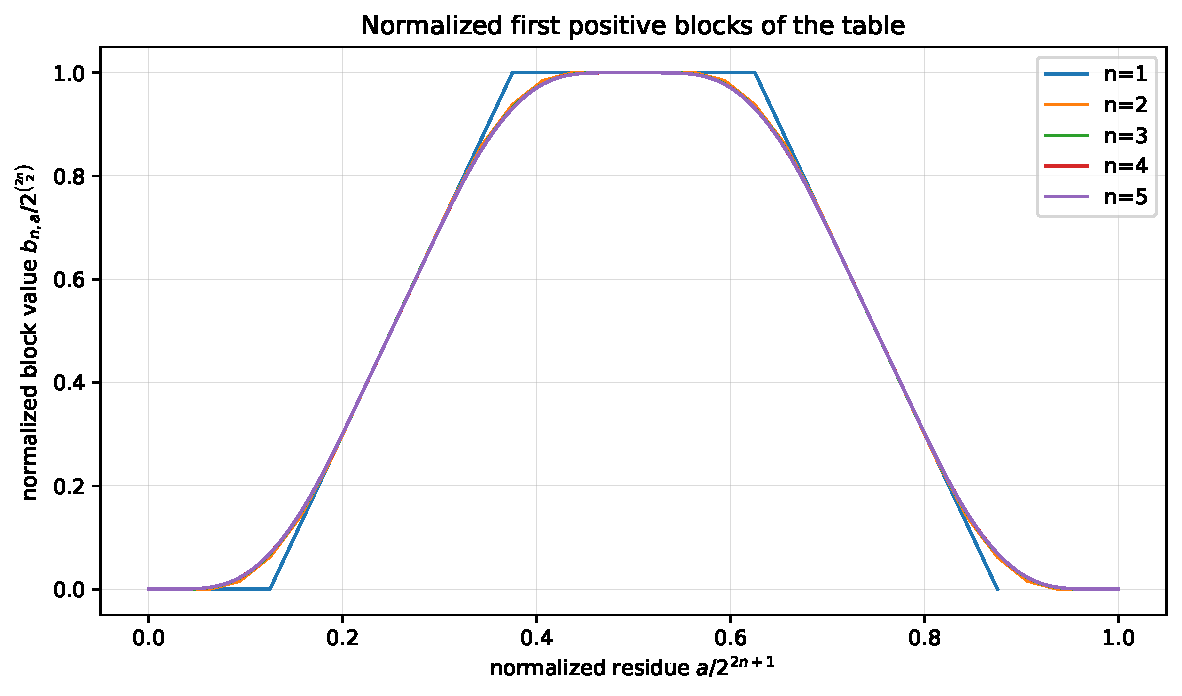
\includegraphics[width=0.94\textwidth]{row_profiles.pdf}
\caption{Normalized first positive blocks for \(n=1,\ldots,5\), generated by
\texttt{experiments.py}.  The central plateau has exact width
\((2n+1)/2^{2n+1}\), and the mirror/complement laws hold before taking a
limit.}
\label{fig:row-profiles}
\end{figure}

\section{Algorithms and Wolfram Language implementation}

\subsection{Replacing the finite list of diagonal rules}

The eight hand-written diagonal branches can be replaced by one exact
definition.  The following Wolfram Language code uses \texttt{Pochhammer} for
the rising factorial and memoizes each symbolic polynomial.

\begin{lstlisting}[language=Mathematica,caption={Exact polynomial for every diagonal.}]
ClearAll[tmSign, diagonalPolynomial, x];

tmSign[q_Integer?NonNegative] := (-1)^ThueMorse[q];

diagonalPolynomial[0] = 1;
diagonalPolynomial[r_Integer?Positive] :=
  diagonalPolynomial[r] =
    Expand@Sum[
      tmSign[q] Pochhammer[2 x, r - 2 q]/Factorial[r - 2 q],
      {q, 0, Quotient[r, 2]}
    ];

ClearAll[sByDiagonal];
sByDiagonal[n_Integer?NonNegative, k_Integer?NonNegative] /; k <= n := 0;
sByDiagonal[n_Integer?NonNegative, k_Integer?NonNegative] :=
  diagonalPolynomial[k - n - 1] /. x -> n;
\end{lstlisting}

This route is ideal when \(k-n\) is small and \(n\) is large: its work depends
on the diagonal offset, not on the row index.  A direct numeric form avoids
symbolic expansion:

\begin{lstlisting}[language=Mathematica,caption={Direct exact evaluation of one diagonal entry.}]
ClearAll[sDiagonalValue];
sDiagonalValue[n_Integer?NonNegative, k_Integer?NonNegative] /; k <= n := 0;
sDiagonalValue[n_Integer?NonNegative, k_Integer?NonNegative] := Module[
  {r = k - n - 1},
  Sum[
    (-1)^ThueMorse[q] Binomial[2 n + r - 2 q - 1, r - 2 q],
    {q, 0, Quotient[r, 2]}
  ]
];
\end{lstlisting}

\subsection{Generating consecutive polynomials by the ruler recurrence}

When all diagonals through \(r=R\) are wanted, the recurrence
\eqref{eq:ruler-recurrence} reuses previous results and exposes the valuation
structure.

\begin{lstlisting}[language=Mathematica,basicstyle=\ttfamily\footnotesize,caption={Ruler-function recurrence for consecutive diagonals.}]
ClearAll[diagonalRuler, x];
diagonalRuler[0] = 1;
diagonalRuler[r_Integer?Positive] :=
  diagonalRuler[r] = Expand[
    Sum[
      (2 x + 2 - 2^(IntegerExponent[m, 2] + 1))
        diagonalRuler[r - m],
      {m, 1, r}
    ]/r
  ];
\end{lstlisting}

The recurrence is triangular and requires \(R(R+1)/2\) polynomial
multiplications by linear factors.  For one isolated diagonal,
\eqref{eq:main-diagonal} is usually shorter; for a full prefix of the family,
the ruler recurrence is usually preferable.

\subsection{Precomputing a complete row block}

For fixed moderate \(n\) and many arbitrary \(k\), precompute the one positive
block \(B_n\) and use the signed block law.

\begin{lstlisting}[language=Mathematica,caption={Block-based exact table lookup.}]
ClearAll[z, rowBlockPolynomial, rowBlock, sByBlock];

rowBlockPolynomial[n_Integer?NonNegative] :=
  rowBlockPolynomial[n] = Expand[
    z^(n + 1) Product[
      Sum[z^a, {a, 0, 2^j - 1}],
      {j, 1, 2 n}
    ]
  ];

rowBlock[n_Integer?NonNegative] := rowBlock[n] = Module[
  {len = 2^(2 n + 1)},
  PadRight[CoefficientList[rowBlockPolynomial[n], z], len]
];

sByBlock[n_Integer?NonNegative, k_Integer?NonNegative] := Module[
  {len = 2^(2 n + 1), q, a},
  q = Quotient[k, len];
  a = Mod[k, len];
  (-1)^ThueMorse[q] rowBlock[n][[a + 1]]
];
\end{lstlisting}

The polynomial expansion shown here is concise and suitable for presentation.
For larger \(n\), the companion Python code computes the same coefficient list
by repeated convolution with all-one windows, using a sliding sum so each
factor is processed in linear time in the current output length.

\subsection{Useful additional acceleration rules}

The structural theorem supplies exact branches that are absent from the
original listing.  Inside the first block and for \(n\ge1\),
\begin{align}
 s_{n,L_n/4}&=M_n/2,
 \label{eq:wl-quarter-rule}\\
 s_{n,a}&=M_n
 \quad\text{for }L_n/2-n\le a\le L_n/2+n,
 \label{eq:wl-plateau-rule}\\
 s_{n,a}&=0
 \quad\text{for }0\le a\le n
 \text{ or }L_n-n\le a<L_n.
 \label{eq:wl-zero-rule}
\end{align}
Together with the stronger full-half complement
\eqref{eq:row-complement}, these can reduce recursion depth substantially.
Care is required to order conditional definitions so that fixed points such as
\(a=L_n/4\) are handled before a symmetry branch referring to themselves.

The standalone file \texttt{thue\_morse\_table.wl} packages these identities in
\texttt{sFast[n,k]}.  It first reduces \(k\) to its signed dyadic block, maps the
local residue through the zero, plateau, reflection, and complement laws into the
first quarter, and finally calls the finite diagonal formula.  Thus an arbitrary
entry can be evaluated without constructing the complete exponentially long block.

\section{Computational verification}

The archive accompanying this article contains
\texttt{experiments.py}.  Its identities are checked with Python integers and
SymPy exact rationals; floating-point arithmetic is used only to draw
Figure~\ref{fig:row-profiles}.  The program performs the following independent
comparisons.

\begin{enumerate}
\item It builds the table from the original weighted recurrence using prefix
sums to evaluate each weighted convolution in constant time after preprocessing
one row.

\item It evaluates \(\Diag_{k-n-1}(n)\) directly from
\eqref{eq:main-diagonal} and compares every tested entry with the recurrence.

\item It constructs the finite block \(B_n\) by sliding-window convolutions
and compares the signed-block lookup with both previous methods.

\item It mirrors the branch order of the Wolfram Language hybrid evaluator
\texttt{sFast}, checks every residue of the tested row blocks, and then checks
several complete signed repetitions.

\item It constructs the same diagonal polynomials independently from the
ruler recurrence and verifies the half-step and differential identities
symbolically.

\item It checks support, reflection, complement, plateau, total mass,
multiplicities, and distinct-value counts for several rows and for arbitrary
summation orders \(h\) through the tested range.

\item It verifies the nonnegative half-integer root criterion and the negative
half-integer finite-difference formula, including the two valuation criteria
\eqref{eq:x-minus-one-root}--\eqref{eq:x-minus-two-root}.
\end{enumerate}

A successful run prints
\begin{lstlisting}
All exact checks passed.
\end{lstlisting}
and writes a text report of the initial factorizations.  These experiments are
regression checks rather than substitutes for the proofs above.

\section{Further deductions and research directions}

\subsection{Polynomial interpolation in a discrete parameter}

The variable \(x\) is not merely a formal row coordinate.  Under
\(h=2x+1\), it continuously interpolates the discrete order of summation.  The
half-step recurrence is exactly the identity that one additional summation in
\(h\) produces one lower-index coefficient after taking a difference in the
order parameter.  This may be useful when comparing different repeated-
integration normalizations in the Fabius corpus.

\subsection{Root automata and residual factors}

The nonnegative half-integer roots are completely classified by a terminal
block condition.  At a fixed negative half-integer, the zero test is a finite
linear combination of a bounded window of Thue--Morse signs.  This suggests a
systematic finite-automaton study of the residual linear factors of
\(\Diag_r\) as \(r\) varies.  The examples \(x+1\) and \(x+2\) already reduce
to elementary \(2\)-adic valuation parity.  Higher backward differences
produce richer but still finite digital conditions.

\subsection{Other Mahler products}

The deflation theorem \eqref{eq:general-deflation} applies whenever a base
generating function contains a factor \((1-z)^c\) and then contracts to
\(z^b\).  For products of the form
\[
 E_b(z)=\prod_{j\ge0}(1-z^{b^j}),
 \qquad
 E_b(z)=(1-z)E_b(z^b),
\]
one obtains an analogous sparse diagonal polynomial with degree gaps in
multiples of \(b\).  Finite-level factorization then produces blocks of length
\(b^h\).  Positivity and the exact plateau geometry require additional care
when the quotient factors are no longer all-one intervals, but the polynomial
mechanism survives unchanged.

\subsection{Formalization targets}

The repository already crosswalks Lean proofs of the exact prefix formula,
iterated-prefix convolution, finite dyadic quotient, terminal zero run, and
signed reversal \cite{ReshetnikovAtlas}.  Natural additions suggested by this
article are:

\begin{enumerate}
\item a polynomial-valued definition of \(\Diag_r\) and the evaluation theorem
\(s_{n,n+1+r}=\Diag_r(n)\);
\item the half-step and ruler recurrences;
\item the exact half-integer zero criterion;
\item the plateau, complement, multiplicity, and distinct-value theorems for
\(Q_h\) and \(B_n\).
\end{enumerate}

Each statement is finite algebra over integer polynomials once the existing
product identities are imported.

\section{Conclusion}

The apparent list of special diagonal formulas is one family:
\[
 \Diag_r(x)=\coeff{r}{E(z^2)(1-z)^{-2x}}.
\]
The Mahler equation compresses this coefficient to the explicit finite sum
\eqref{eq:main-diagonal}; the resulting polynomial has exact degree \(r\), a
controlled Stirling coefficient structure, half-lattice integrality, and a
Sheffer calculus governed by the binary ruler function.  Its nonnegative
half-integer factors are precisely the terminal-zero positions of iterated
Thue--Morse blocks.

At the global level, each row is not merely approximately periodic in shape:
it is an exact signed concatenation of one finite positive block.  The support,
reflection, complement, plateau, maximum, mass, and multiplicity laws all
follow from splitting one geometric factor from a finite Prouhet quotient.
This gives both a conceptual description of the two-dimensional table and
practical exact algorithms tailored to either fixed diagonals or arbitrary
large columns.

\appendix

\section{A compact theorem dictionary}

For reference, the principal objects and translations are collected here.

\begin{center}
\begin{tabularx}{\textwidth}{@{}p{0.25\textwidth}X@{}}
\toprule
Object & Exact formula or relation \\
\midrule
Signed Thue--Morse & \(\eps_q=(-1)^{\wt(q)}\) \\
Lacunary series & \(E(z)=\sum_q\eps_qz^q=\prod_{j\ge0}(1-z^{2^j})\) \\
Mahler equation & \(E(z)=(1-z)E(z^2)\) \\
Exclusive prefix & \(S(2q)=0,\ S(2q+1)=\eps_q\) \\
Iterated prefix & \(\sum_r\Prefix_r^{(h)}z^r=E(z)/(1-z)^h\) \\
Row generating function & \(A_n(z)=z^{n+1}E(z)/(1-z)^{2n+1}\) \\
Row/prefix map & \(s_{n,n+1+r}=\Prefix_r^{(2n+1)}\) \\
Diagonal polynomial & \(\Diag_r(x)=[z^r]E(z^2)/(1-z)^{2x}\) \\
Original diagonal \(d\) & \(P_d(x)=\Diag_{d-1}(x)\) \\
Half-step & \(\Diag_r(x)-\Diag_r(x-1/2)=\Diag_{r-1}(x)\) \\
Ruler coefficient & \(c_m(x)=2x+2-2^{\nuTwo(m)+1}\) \\
Ruler recurrence & \(r\Diag_r=\sum_{m=1}^rc_m\Diag_{r-m}\) \\
Row block length & \(L_n=2^{2n+1}\) \\
Row maximum & \(M_n=2^{\binom{2n}{2}}\) \\
Signed block law & \(s_{n,qL_n+a}=\eps_qb_{n,a}\) \\
\bottomrule
\end{tabularx}
\end{center}

\section{Reproducibility files}

The source archive contains:
\begin{itemize}
\item \texttt{thue\_morse\_diagonal\_polynomials.tex}, this source;
\item \texttt{thue\_morse\_diagonal\_polynomials.pdf}, the rendered article;
\item \texttt{experiments.py}, fully commented exact verification code;
\item \texttt{thue\_morse\_table.wl}, a standalone Wolfram Language
implementation of the diagonal, ruler, hybrid, and block algorithms;
\item \texttt{verification\_report.txt}, output from a successful run;
\item \texttt{row\_profiles.pdf} and \texttt{row\_profiles.png}, the generated
figure in vector and raster form;
\item \texttt{README.txt}, build and execution instructions;
\item \texttt{SHA256SUMS}, cryptographic checksums for the packaged files.
\end{itemize}

\clearpage
\begin{thebibliography}{99}

\bibitem{AlloucheShallit}
J.-P. Allouche and J. Shallit,
\emph{Automatic Sequences: Theory, Applications, Generalizations},
Cambridge University Press, 2003.

\bibitem{Bertazzon2012}
J.-F. Bertazzon,
``Resolution of an integral equation with the Thue--Morse sequence,''
\emph{arXiv:1201.2502 [math.CO]}, 2012.
\url{https://arxiv.org/abs/1201.2502}

\bibitem{Comtet1974}
L. Comtet,
\emph{Advanced Combinatorics: The Art of Finite and Infinite Expansions},
D. Reidel, 1974.

\bibitem{Fabius1966}
J. Fabius,
``A probabilistic example of a nowhere analytic \(C^\infty\)-function,''
\emph{Zeitschrift f\"ur Wahrscheinlichkeitstheorie und Verwandte Gebiete},
vol.~5, 1966, pp.~173--174.

\bibitem{ReshetnikovMSE}
V. Reshetnikov,
``Periodic sequences resulting from a summation over the Thue--Morse
sequence,'' Mathematics Stack Exchange, question 2784373, 2018.
\url{https://math.stackexchange.com/questions/2784373/periodic-sequences-resulting-from-a-summation-over-the-thue-morse-sequence}

\bibitem{ReshetnikovAtlas}
V. Reshetnikov,
\emph{The Thue--Morse Sequence: Formula Atlas and Fabius--Rvachev Frontier
Results}, consolidated research manuscript in the \texttt{ProveIt}
repository, 28 August 2026; accessed 3 September 2026.
\url{https://github.com/VladimirReshetnikov/ProveIt/tree/main/Analysis/FabiusFunction/docs/semi-formalized-research-frontiers/drafts/thue-morse/Thue_Morse_Atlas_and_Frontiers}

\bibitem{Roman1984}
S. Roman,
\emph{The Umbral Calculus},
Academic Press, 1984.

\bibitem{Rvachev1990}
V. A. Rvachev,
``Compactly supported solutions of functional-differential equations and
their applications,''
\emph{Russian Mathematical Surveys}, vol.~45, no.~1, 1990, pp.~87--120.

\end{thebibliography}

\end{document}
